\subsection*{Explicación}
Un JK-flip-flop hace lo mismo que un JK-latch excepto que lo realiza en los posedge del clock.

\subsection*{Tabla de verdad}
\begin{figure}[h]
    \centering
    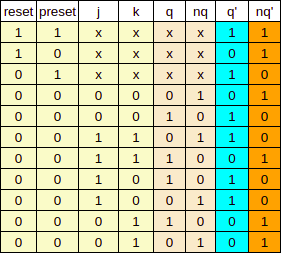
\includegraphics{fotos/TruthTable/arki-lab2-TT_jkflipflop.png}
\end{figure}
%\subsection*{Mapa de Karnaugh}
%\begin{figure}[h]
%    \centering

%\end{figure}

%\subsection*{Ecuaciones booleanas}


%\subsection*{Resultados}
%\begin{figure}[h]
%    \centering

%\end{figure}
